\documentclass[aspectratio=169]{beamer}
\usepackage[utf8]{inputenc}
\usepackage{hyperref}
\usepackage{amsmath,amsfonts,amsthm,bm}
\usepackage{color}
\usepackage{minted}
\usepackage{graphicx} % Allows including images
\usepackage{subcaption}
\usepackage{booktabs} % Allows the use of \toprule, \midrule and \bottomrule in tables
\usepackage{tikz}
%\usepackage{pgfplots}
\usepackage{listings}
\usepackage{courier}
\usepackage[version=4]{mhchem}
\usepackage{array}
\setminted{fontsize=\scriptsize}
\lstset{ %
    basicstyle=\scriptsize\ttfamily, % fonts that are used for the code
    breakatwhitespace=false,         % sets if automatic breaks should only happen at whitespace
%breaklines=true,                 % sets automatic line breaking
%captionpos=b,                    % sets the caption-position to bottom
    commentstyle=\color{gray}\textit,    % comment style
    keepspaces=true,                 % keeps spaces in text, useful for keeping indentation of code (possibly needs columns=flexible)
    keywordstyle=\color{blue},       % keyword style
    language=Python,                 % the language of the code
%otherkeywords={*,...},          % if you want to add more keywords to the set
    rulecolor=\color{black},         % if not set, the frame-color may be changed on line-breaks within not-black text (e.g. comments (green here))
    showspaces=false,                % show spaces everywhere adding particular underscores; it overrides 'showstringspaces'
    showstringspaces=false,          % underline spaces within strings only
    showtabs=false,                  % show tabs within strings adding particular underscores
    stringstyle=\color{red}, % string literal style
    tabsize=4,                       % sets default tabsize to 2 spaces
    columns=fixed                    % Using fixed column width (for e.g. nice alignment)
}

\hypersetup{
    colorlinks=true,
    linkcolor=red,
    filecolor=magenta,
    urlcolor=red,
}

\DeclareMathOperator*{\argmax}{argmax}
\DeclareMathOperator*{\argmin}{argmin}
\let \vec \mathbf

\newcommand{\classname}{NANO266}
\newcommand{\classyear}{Fall 2024}
\mode<presentation> {
    \usetheme{CambridgeUS}
    \setbeamertemplate{footline}[text line]{%
        \parbox{\linewidth}{\vspace*{-8pt}\classname\hfill\classyear\hfill\insertpagenumber}}

    %\setbeamertemplate{footline}[page number]
    \setbeamertemplate{navigation symbols}{}
}


\title[\classname Lab 4 - Surface Properties of Aluminum]{\classname~- Quantum Mechanical Modeling of Materials and Nanostructures\\Lab 4 - Surface Properties of Aluminum}

\author{Shyue Ping Ong}
\institute[UCSD]{University of California, San Diego\\
\medskip
}
\date{\classyear} % Date, can be changed to a custom date

\begin{document}


    \begin{frame}
        \titlepage % Print the title page as the first slide
    \end{frame}


    \begin{frame}{Aims of Lab 3}
        \Large{
            \begin{enumerate}
                \item Understand how to model surfaces using DFT.
                \item Construction of surface models using VESTA.
                \item Investigate the binding of atoms on differents sites on Al surface.
            \end{enumerate}
        }
    \end{frame}

    \begin{frame}{Aluminum}
        \begin{columns}
            \column{0.8\textwidth}
            The most widely used metal in the world after iron.
            \begin{itemize}
                \item Global production in 2016: 58.8 million metric tons.
                \item Lower density than other common metals ($\approx 1/3$ of steel).
                \item Corrosion resistant (due to formation of protective layer of oxide).
                \item Many applications in transportation, packaging, construction, household items, etc.
            \end{itemize}

            \column{0.2\textwidth}
            \begin{figure}
                \centering
                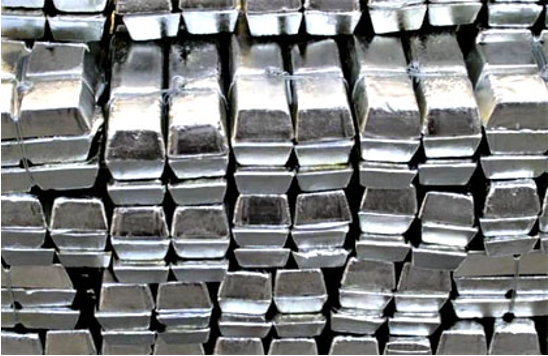
\includegraphics[width=0.8\linewidth]{lectures/figures/Lab4_Al1.png}
                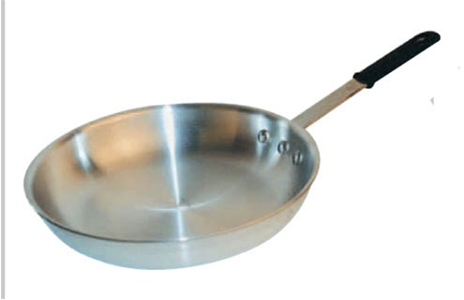
\includegraphics[width=0.8\linewidth]{lectures/figures/Lab4_Al2.png}
                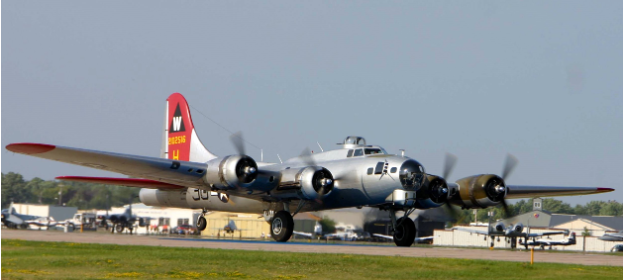
\includegraphics[width=0.8\linewidth]{lectures/figures/Lab4_Al3.png}
                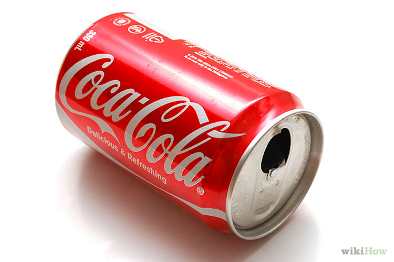
\includegraphics[width=0.8\linewidth]{lectures/figures/Lab4_Al4.png}
            \end{figure}

        \end{columns}

    \end{frame}

    \begin{frame}{Low-index surfaces of fcc crystals}

        \begin{figure}
            \centering
            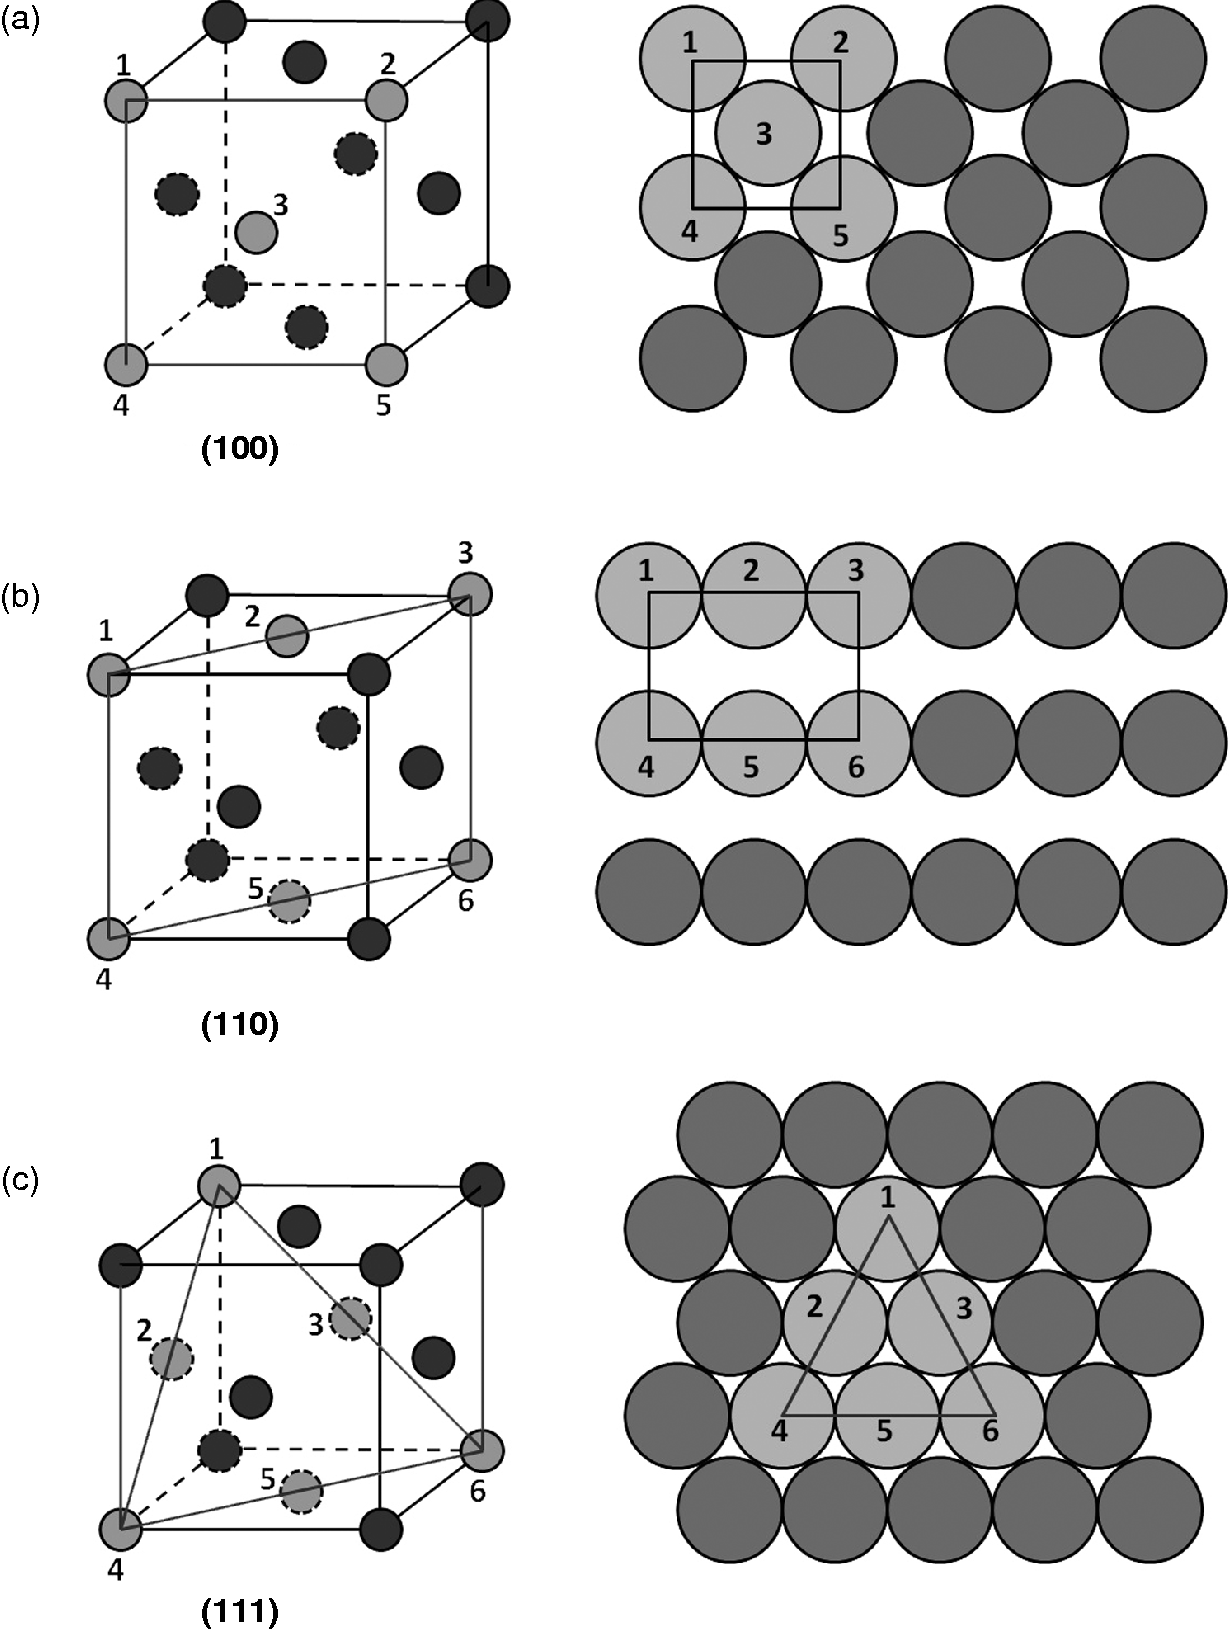
\includegraphics[width=0.3\linewidth]{lectures/figures/Lab4_fcc_surfaces.png}
        \end{figure}
    \end{frame}

    \begin{frame}{Modelling surfaces with the Supercell method}

        \begin{figure}
            \centering
            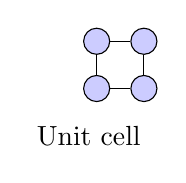
\begin{tikzpicture}[scale=0.5,
                atom/.style={circle,draw=black,fill=white!80!blue,minimum size=5},
                dopant/.style={circle,draw=black,fill=white!80!red,minimum size=5}
            ]
                \foreach \i in {1,...,2}
                    {
                    \foreach \j in {1,...,2}
                        {
                        \pgfmathtruncatemacro{\label}{\i\j};
                        \node[atom] (\label) at (1.2*\i,1.2*\j) { };

                    }
                }
% These draw commands are working as intended.
                \draw (11) -- (12);
                \draw (12) -- (22);
                \draw (21) -- (22);
                \draw (11) -- (21);
                \node at (1, 0) { Unit cell };

            \end{tikzpicture}
        \end{figure}

    \end{frame}


    \begin{frame}{Modelling surfaces with the Supercell method}

        \begin{figure}
            \centering
            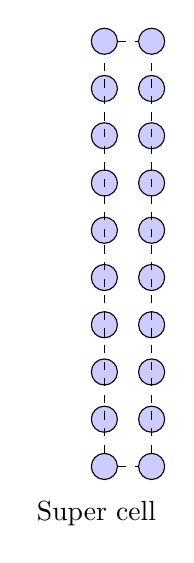
\begin{tikzpicture}[scale=0.5,
                atom/.style={circle,draw=black,fill=white!80!blue,minimum size=5},
                dopant/.style={circle,draw=black,fill=white!80!red,minimum size=5}
            ]
                \foreach \i in {1,...,2}
                    {
                    \foreach \j in {1,...,10}
                        {
                        \pgfmathtruncatemacro{\label}{\i\j};
                        \node[atom] (\label) at (1.2*\i,1.2*\j) { };
                    }
                }
                \draw[dashed] (11) -- (110);
                \draw[dashed] (11) -- (21);
                \draw[dashed] (21) -- (210);
                \draw[dashed] (110) -- (210);
                \node at (1, 0) { Super cell };

            \end{tikzpicture}
        \end{figure}

    \end{frame}


    \begin{frame}{Modelling surfaces with the Supercell method}

        \begin{figure}
            \centering
            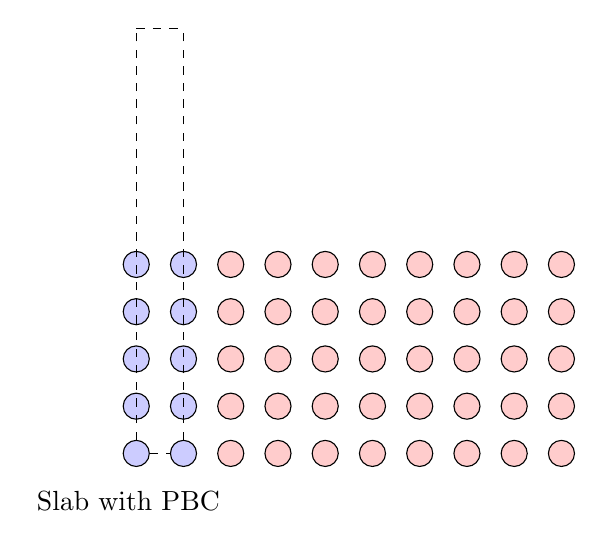
\begin{tikzpicture}[scale=0.5,
                atom/.style={circle,draw=black,fill=white!80!blue,minimum size=5},
                dopant/.style={circle,draw=black,fill=white!80!red,minimum size=5}
            ]
                \foreach \i in {1,...,2}
                    {
                    \foreach \j in {1,...,5}
                        {
                        \pgfmathtruncatemacro{\label}{\i\j};
                        \node[atom] (\label) at (1.2*\i,1.2*\j) { };
                    }
                }
                \foreach \i in {3,...,10}
                    {
                    \foreach \j in {1,...,5}
                        {
                        \pgfmathtruncatemacro{\label}{\i\j};
                        \node[dopant] (\label) at (1.2*\i,1.2*\j) { };
                    }
                }
                \draw[dashed] (11) -- (1.2,12);
                \draw[dashed] (11) -- (21);
                \draw[dashed] (21) -- (2.4,12);
                \draw[dashed] (1.2,12) -- (2.4,12);
                \node at (1, 0) { Slab with PBC };

            \end{tikzpicture}
        \end{figure}

    \end{frame}

    \begin{frame}{Convergence of Surface Energies}
        \begin{columns}
            \column{0.3\textwidth}
            \begin{figure}
                \centering
                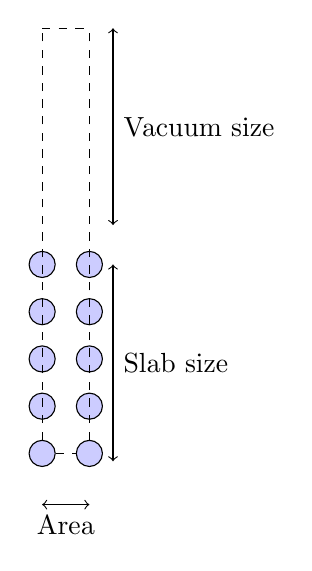
\begin{tikzpicture}[scale=0.5,
                    atom/.style={circle,draw=black,fill=white!80!blue,minimum size=5},
                    dopant/.style={circle,draw=black,fill=white!80!red,minimum size=5}
                ]
                    \foreach \i in {1,...,2}
                        {
                        \foreach \j in {1,...,5}
                            {
                            \pgfmathtruncatemacro{\label}{\i\j};
                            \node[atom] (\label) at (1.2*\i,1.2*\j) { };
                        }
                    }

                    \draw[dashed] (11) -- (1.2,12);
                    \draw[dashed] (11) -- (21);
                    \draw[dashed] (21) -- (2.4,12);
                    \draw[dashed] (1.2,12) -- (2.4,12);
                    \draw[<->] (3,1) -- node[right= 0.1mm] {Slab size} (3, 6);
                    \draw[<->] (3,7) -- node[right= 0.1mm] {Vacuum size} (3, 12);
                    \draw[<->] (1.2,-0.1) -- node[below= 0.1mm] {Area} (2.4, -0.1);

                \end{tikzpicture}
            \end{figure}
            \column{0.7\textwidth}
            \begin{equation*}
                \gamma = \frac{1}{2A} [ E(\mathrm{slab})-NE(\mathrm{bulk})]
            \end{equation*}

        \end{columns}
    \end{frame}
    \begin{frame}{Making the surface models}
        \begin{itemize}
            \item (100): Trivial since the cube face is already the (100) surface. Extend cube in one direction (e.g., $c$) and delete atoms.
            \item (111): Need to perform lattice transformation to get cell with (111) surface as one of the faces before extending the cell. Detailed instructions are given on the \href{https://github.com/materialsvirtuallab/nano266/tree/master/labs/lab4}{Github repo}.
        \end{itemize}
    \end{frame}

    \begin{frame}{Important: CPU usage}
        Keep track of your CPU usage.\newline
        \newline
        Do NOT exceed 1000 SUs. (You can calculate your SUs by simply summing the time for your runs, since we are running only single-processor jobs).
    \end{frame}


% \begin{frame}[allowframebreaks]{Bibliography}
%     \bibliographystyle{unsrt}
%     \bibliography{refs}
% \end{frame}

    \begin{frame}
        \Huge{\centerline{The End}}
    \end{frame}

\end{document}

